\documentclass[11pt,a4paper]{article}
% Shared preamble for the NAIL094 reports
% Used by every task via % Shared preamble for the NAIL094 reports
% Used by every task via % Shared preamble for the NAIL094 reports
% Used by every task via \input{../../shared/preamble}

\usepackage[T1]{fontenc}
\usepackage[utf8]{inputenc}
\usepackage{lmodern}
\usepackage[margin=2.5cm]{geometry}

\usepackage{amsmath}
\usepackage{amssymb}
\usepackage{booktabs}
\usepackage{float}
\usepackage{graphicx}
\usepackage{listings}
\usepackage{xcolor}
\usepackage{caption}

\usepackage[hidelinks]{hyperref}

\setlength{\parskip}{0.5em}
\setlength{\parindent}{0pt}

% Title fields, set these in the report before \begin{document}
\makeatletter
\newcommand{\reportcourse}[1]{\def\@reportcourse{#1}}
\newcommand{\reporttask}[1]{\def\@reporttask{#1}}
\newcommand{\reportauthor}[1]{\def\@reportauthor{#1}}

\newcommand{\makereporttitle}{%
  \begin{center}
    {\LARGE\bfseries \@reportcourse \par}
    \vspace{0.8em}
    {\Large \@reporttask \par}
    \vspace{0.6em}
    {\normalsize \@reportauthor \par}
  \end{center}
  \vspace{1em}
  \hrule
  \vspace{1.5em}
}
\makeatother

% Inline code
\newcommand{\code}[1]{\texttt{#1}}

% Code listings
\lstdefinestyle{reportcode}{
  basicstyle=\ttfamily\small,
  keywordstyle=\color{blue!60!black},
  commentstyle=\color{gray},
  stringstyle=\color{green!40!black},
  breaklines=true,
  showstringspaces=false,
  frame=single,
  rulecolor=\color{gray!40},
  numbers=none,
}
\lstset{style=reportcode}


\usepackage[T1]{fontenc}
\usepackage[utf8]{inputenc}
\usepackage{lmodern}
\usepackage[margin=2.5cm]{geometry}

\usepackage{amsmath}
\usepackage{amssymb}
\usepackage{booktabs}
\usepackage{float}
\usepackage{graphicx}
\usepackage{listings}
\usepackage{xcolor}
\usepackage{caption}

\usepackage[hidelinks]{hyperref}

\setlength{\parskip}{0.5em}
\setlength{\parindent}{0pt}

% Title fields, set these in the report before \begin{document}
\makeatletter
\newcommand{\reportcourse}[1]{\def\@reportcourse{#1}}
\newcommand{\reporttask}[1]{\def\@reporttask{#1}}
\newcommand{\reportauthor}[1]{\def\@reportauthor{#1}}

\newcommand{\makereporttitle}{%
  \begin{center}
    {\LARGE\bfseries \@reportcourse \par}
    \vspace{0.8em}
    {\Large \@reporttask \par}
    \vspace{0.6em}
    {\normalsize \@reportauthor \par}
  \end{center}
  \vspace{1em}
  \hrule
  \vspace{1.5em}
}
\makeatother

% Inline code
\newcommand{\code}[1]{\texttt{#1}}

% Code listings
\lstdefinestyle{reportcode}{
  basicstyle=\ttfamily\small,
  keywordstyle=\color{blue!60!black},
  commentstyle=\color{gray},
  stringstyle=\color{green!40!black},
  breaklines=true,
  showstringspaces=false,
  frame=single,
  rulecolor=\color{gray!40},
  numbers=none,
}
\lstset{style=reportcode}


\usepackage[T1]{fontenc}
\usepackage[utf8]{inputenc}
\usepackage{lmodern}
\usepackage[margin=2.5cm]{geometry}

\usepackage{amsmath}
\usepackage{amssymb}
\usepackage{booktabs}
\usepackage{float}
\usepackage{graphicx}
\usepackage{listings}
\usepackage{xcolor}
\usepackage{caption}

\usepackage[hidelinks]{hyperref}

\setlength{\parskip}{0.5em}
\setlength{\parindent}{0pt}

% Title fields, set these in the report before \begin{document}
\makeatletter
\newcommand{\reportcourse}[1]{\def\@reportcourse{#1}}
\newcommand{\reporttask}[1]{\def\@reporttask{#1}}
\newcommand{\reportauthor}[1]{\def\@reportauthor{#1}}

\newcommand{\makereporttitle}{%
  \begin{center}
    {\LARGE\bfseries \@reportcourse \par}
    \vspace{0.8em}
    {\Large \@reporttask \par}
    \vspace{0.6em}
    {\normalsize \@reportauthor \par}
  \end{center}
  \vspace{1em}
  \hrule
  \vspace{1.5em}
}
\makeatother

% Inline code
\newcommand{\code}[1]{\texttt{#1}}

% Code listings
\lstdefinestyle{reportcode}{
  basicstyle=\ttfamily\small,
  keywordstyle=\color{blue!60!black},
  commentstyle=\color{gray},
  stringstyle=\color{green!40!black},
  breaklines=true,
  showstringspaces=false,
  frame=single,
  rulecolor=\color{gray!40},
  numbers=none,
}
\lstset{style=reportcode}


\reportcourse{NAIL094 --- Decision Procedures and SAT/SMT Solvers}
\reporttask{Backbones}
\reportauthor{Zerina Ahmetovic}

\begin{document}
\makereporttitle

\section{Task overview}

A literal $l$ is a backbone of $\varphi$ if $l$ is in every model of
$\varphi$, or in other words the value of $l$ is implied by $\varphi$, that is
$\varphi \models l$. The task is to write a program which uses a SAT solver as
an oracle and finds all backbones of a given CNF $\varphi$. The CNF is given
in DIMACS format.

A strategy or heuristic has to be used to minimise the number of SAT calls. Further, if a
formula is satisfiable the SAT solver can return a model, and the information
given by that model is to be used to minimise the number of SAT calls.

The program has to be evaluated on several SATLIB benchmark
problems~\cite{satlib}.

\section{Analysis}

\subsection*{Reduction to satisfiability}

A literal $l$ is a backbone only when $\varphi \wedge \neg l$ has no model,
so a single unsatisfiable answer confirms one backbone. Testing every literal
this way gives the naive algorithm: for each variable $x$ ask whether
$\varphi \wedge x$ is unsatisfiable, in which case $\neg x$ is a backbone, and
otherwise ask whether $\varphi \wedge \neg x$ is unsatisfiable, in which case
$x$ is one. If none works, proceed to the next variable. This costs $2n$ calls for $n$ variables, and it is the baseline
that both algorithms below are measured against.

\subsection*{Shortcut halving the work}

If $\varphi$ is satisfiable then $x$ and $\neg x$ cannot both be backbones,
since a model would have to contain both. Take any model $M$ of $\varphi$.
For every variable $x$, $M$ already witnesses one polarity: if $M$ sets $x$
true then $M$ is a model in which $x$ holds, so $\neg x$ is not a backbone.

Only the polarity that $M$ agrees with remains a candidate. One call, made
once at the start, therefore removes half of the $2n$ literals, and the
remaining test for each variable is the one that has a chance of failing. The
other test is guaranteed to succeed and would be wasted. This is what the task
means by using the information given by the model.

The same argument applies to every later model. Whenever a test returns
satisfiable, the model it returns falsifies some candidates, and all of them
can be discarded at once rather than only the literal being tested.

\subsection*{Instant backbones (unit propagation)}

Any unit clause $(l)$ of $\varphi$ is satisfied only when $l$ holds (since $\varphi$ is in CNF), so $l$ is
a backbone without any test at all. More generally, if $\varphi \models l_1$
and unit propagation from $l_1$ derives $l_2$, then $\varphi \models l_2$, so
everything the propagation closure produces is a backbone as well.

This combines with the observation that a confirmed backbone can be added to
the formula as a unit clause, since $\varphi \models l$ means
$\varphi \equiv \varphi \wedge l$. Committing a backbone therefore strengthens
the formula for every later call and may cascade into further backbones at no
cost. The propagation is done in the program itself and involves no solver, so
these literals are truly free in the sense of the metric being reported.

\subsection*{The two algorithms}

Both start from one model and both use the propagation closure. They
differ in how the remaining candidates are decided.

\paragraph{Algorithm \code{propagate}.}
One call per candidate. For each remaining candidate $l$, ask whether
$\varphi \wedge \neg l$ is satisfiable. If it is not, $l$ is a backbone, it is
committed into the formula and its propagation closure is derived. If it is,
$l$ is not a backbone and the returned model is used to discard every other
candidate it falsifies. The number of calls is bounded by the number of
candidates, so at most $n$.

\paragraph{Algorithm \code{complement}.}
One call per pruning round. Instead of asking about a single literal, ask for
a model that falsifies at least one remaining candidate, by adding the clause
$\bigvee_{l \in C} \neg l$ over the current candidate set $C$. There are two
outcomes:
\begin{itemize}
  \item satisfiable: the model falsifies one or more candidates, and all of
  them are removed at once, so a single call can prune many literals;
  \item unsatisfiable: no model of $\varphi$ falsifies any candidate, which
  means every remaining candidate is a backbone and the search ends.
\end{itemize}
The clause has to be replaced on every round, so it is added guarded by a
fresh selector variable $s$ as $\neg s \vee \bigvee_{l \in C} \neg l$,
activated by assuming $s$ and retired afterwards by asserting $\neg s$. The
number of calls is the number of rounds, which is bounded by the number of
candidates but in practice far smaller.

\subsection*{Edge cases}

If $\varphi$ is unsatisfiable then $\varphi \models l$ holds vacuously for
every literal, so all $2n$ literals are backbones. Both algorithms detect this
on the very first call and report it, rather than looping through the
variables and finding every test unsatisfiable. A formula with no clauses has
no backbones, and a formula whose backbone is empty, which happens whenever
the models are symmetric enough, is handled without any special casing.

\subsection*{Correctness}
\label{sec:correctness}

The algorithms are sound on paper, but both of them are self reinforcing,
which is why they are checked externally. The first commits confirmed
backbones into the formula, so a literal wrongly accepted early would make
every later answer agree with the mistake. The second concludes that a whole
set of candidates are backbones from one unsatisfiable answer, so an error in
the blocking clause would produce a confident wrong result. Neither failure
shows up as an inconsistency the program could notice on its own.

Four checks are therefore made, all of them outside the measured code and
using their own solver instances, so that no call made while checking is ever
counted:

\begin{itemize}
  \item \textbf{Hand checks.} Small formulas whose backbones can be written
  down by inspection, including the unsatisfiable case, where every one of the
  $2n$ literals is a backbone vacuously.
  \item \textbf{CBS sizes.} The Controlled Backbone Size family of SATLIB
  fixes the number of backbone variables and states it in the file name, which
  is external ground truth on the size.
  \item \textbf{CBS literals.} On the same instances, confirming in addition
  that each reported literal really is a backbone. Since the family fixes the
  size at $b$ and the program reports $b$ literals, a set of $b$ confirmed
  backbones inside a backbone of size $b$ must be the whole of it, so the
  reported set is proved to be the right one and not merely the right size.
  \item \textbf{Full recomputation.} Every instance of the benchmark set,
  described in Section~\ref{sec:verify}, where the backbone is recomputed from
  scratch and compared literal by literal with what each algorithm reported.
\end{itemize}

The distinction between the size and the set matters. Agreeing on how many
backbones there are is weaker than agreeing on which they are, and the first
three checks on their own leave room for a program that reports the right
number of wrong literals. The last check removes that possibility.

\section{Performance analysis}

\subsection*{Solvers}

Every measurement uses CaDiCaL 1.5.3~\cite{cadical}, reached through the PySAT
toolkit~\cite{pysat}, which names it \code{cadical153}. Both
algorithms use the assumption interface, the first to ask about $\neg l$
without changing the formula and the second to activate and retire the
blocking clause.

\subsection*{Setup}

All measurements were taken on a single local machine, an Intel Core
i7-13700H with 16\,GB of memory running Windows 11, under Python 3.11.9
with python-sat 1.9.dev7. The reported quantity is the number of calls to the
solver, since that is what the task asks to minimise. Times are reported as
well, split into loading the formula into the solver and searching. Unit
propagation is performed inside the program and involves no solver, so it adds
nothing to the call count.

The naive algorithm is not run. Its cost is $2n$ calls, fixed by the
number of variables, so measuring it would add nothing that cannot be computed.

\subsection*{Benchmarks}

An unsatisfiable formula entails every literal, so all $2n$ literals would be
backbones vacuously and nothing would be measured. Only families that
SATLIB~\cite{satlib} describes as containing exclusively satisfiable formulas
were therefore used.
They are collected in a shared folder so that other tasks can reuse them, and
every instance was confirmed satisfiable before use.

\begin{table}[H]
\centering
\begin{tabular}{lrrrr}
\toprule
family & instances & variables & clauses & backbone \\
\midrule
\code{uf20-91} & 5 & 20 & 91 & 12.8 \\
\code{uf50-218} & 5 & 50 & 218 & 38.8 \\
\code{flat30-60} & 5 & 90 & 300 & 0.0 \\
\code{BMS\_k3\_n100\_m429} & 5 & 100 & 308 & 29.0 \\
\code{RTI\_k3\_n100\_m429} & 5 & 100 & 429 & 29.0 \\
\code{uf100-430} & 5 & 100 & 430 & 30.0 \\
CBS, 15 families & 75 & 100 & 403--449 & 10--90 \\
\code{flat50-115} & 5 & 150 & 545 & 0.0 \\
\code{ais} & 4 & 265 & 5\,666 & 1.2 \\
\code{flat100-239} & 5 & 300 & 1\,117 & 0.0 \\
\code{sw100-8-p0-c5} & 1 & 500 & 3\,100 & 0.0 \\
\code{logistics} & 4 & 4\,713 & 21\,991 & 559.2 \\
\code{blocksworld} & 7 & 6\,325 & 131\,973 & 1590.7 \\
\bottomrule
\end{tabular}
\caption{The 27 families used, 131 instances in total. Variables and clauses
are the largest in the family, the backbone column is the mean size found.}
\label{tab:bench}
\end{table}

The fifteen CBS families deserve separate mention. They are random 3-SAT
instances generated with a prescribed backbone size~\cite{cbs}, from $b10$
with ten backbone variables to $b90$ with ninety, at three clause counts. They
give both a controlled experiment and the ground truth used to check the
results.

Each of the 131 instances was run with both algorithms, giving 262 runs. None
failed.

\subsection*{Results of the four checks}
\label{sec:verify}

The four checks listed under Correctness in Section~\ref{sec:correctness} all
pass, taken here in the same order.

\emph{Hand checks.} The small formulas give the sets written down by
inspection, and the unsatisfiable formula is reported as having all $2n$
literals as backbones.

\emph{CBS sizes.} Across the 150 runs on the 75 CBS instances the reported
backbone size matched the size stated by the family every time.

\emph{CBS literals.} On those same instances every reported literal was
confirmed to be a backbone, which pins down the set and not only its size.

\emph{Full recomputation.} For every one of the 131 instances the backbone was
recomputed from scratch by testing each of the $2n$ literals with its own
assumption, and the result was compared literal by literal with what each
algorithm reported. Over the 262 comparisons the reported set was identical to
the recomputed one in every case, with no literal missing and none reported in
error. This is the strongest of the four, being the only one that covers the
whole benchmark set.

\begin{table}[H]
\centering
\begin{tabular}{lrr}
\toprule
& calls & counted in the tables below \\
\midrule
\code{propagate} over all instances & 7\,083 & yes \\
\code{complement} over all instances & 6\,367 & yes \\
recomputing the backbone for checking & 64\,541 & no \\
\bottomrule
\end{tabular}
\caption{The verification is deliberately expensive and is kept out of the
measurements. It runs in \code{verify.py}, which builds its own solvers.}
\label{tab:verify}
\end{table}

Table~\ref{tab:verify} also gives an unintended but useful result. The
verification tests every literal with no shortcuts, which is the naive
algorithm, so its $64\,541$ calls are a measurement of the baseline that the
rest of the report only computes as $2n$. The two figures agree, $64\,541$
against a predicted $64\,410$, the small excess being the one satisfiability
call made per instance before the literals are tested.

Independently of all this, the two algorithms agree with each other on all 131
instances, compared on the literals rather than on their number. They arrive
at the answer by completely different routes, one literal at a time against
one round at a time, so an error would have to occur twice over to escape
this comparison.

\subsection*{Solver calls}

\begin{table}[H]
\centering
\begin{tabular}{lrrrrrrrr}
\toprule
& & \multicolumn{3}{c}{calls} & free & \multicolumn{2}{c}{time [s]} & \\
\cmidrule(lr){3-5} \cmidrule(lr){7-8}
algorithm & runs & total & median & max & literals & load & solve & vs naive \\
\midrule
\code{propagate} & 131 & 7\,083 & 32 & 1\,354 & 13\,477 & 0.49 & 63.14 & 9.1 \\
\code{complement} & 131 & 6\,367 & 25 & 2\,395 & 0 & 0.47 & 30.08 & 10.1 \\
\bottomrule
\end{tabular}
\caption{Totals over all 131 instances. The naive algorithm would use
$64\,410$ calls on the same set.}
\label{tab:cost}
\end{table}

Table~\ref{tab:cost} gives the main result. Both algorithms beat the naive
$2n$ comfortably and by similar margins: \code{propagate} uses $9.1$ times
fewer calls and \code{complement} $10.1$ times fewer. Between the two the
difference in calls is small, $7\,083$ against $6\,367$, so neither is the
better choice on the whole set and the comparison has to be made per family
rather than in total. Search time still favours \code{complement}, at
$30.1$ seconds against $63.1$, which says that the calls \code{propagate}
makes are individually dearer: assuming a single literal leaves the solver to
search a nearly unconstrained formula, while the blocking clause of
\code{complement} cuts the space it has to consider.

The free column shows the effect of unit propagation. Of all the backbones
found by \code{propagate}, $13\,477$ literals were obtained without any solver
call. Every one of them comes from the closure of a committed backbone and
none from the units of the input, since no instance in the benchmark set
contains a unit clause at all. Both algorithms run the same initial
propagation and so both derive nothing from it; the column is zero for
\code{complement} because it never commits a literal during the search, and
committing is what gives propagation something to work from.

\subsection*{Calls against backbone size}

\begin{table}[H]
\centering
\begin{tabular}{rrrr}
\toprule
backbone size & \code{propagate} & \code{complement} & naive \\
\midrule
10 & 27.3 & 51.9 & 200 \\
30 & 39.7 & 35.6 & 200 \\
50 & 43.3 & 24.5 & 200 \\
70 & 38.7 & 21.9 & 200 \\
90 & 25.1 & 11.1 & 200 \\
\bottomrule
\end{tabular}
\caption{Mean calls on the CBS instances, 100 variables, averaged over the
three clause counts.}
\label{tab:cbs}
\end{table}

Table~\ref{tab:cbs} is the experiment the CBS family exists for. The number of
variables is fixed at 100 and only the number of forced variables changes, so
the naive cost stays at 200 throughout. The two algorithms answer differently.
\code{complement} falls steadily as the backbone grows, from $51.9$ calls at
ten forced variables to $11.1$ at ninety, while \code{propagate} is cheapest
at both ends and dearest in the middle, rising from $27.3$ to a peak of $43.3$
at fifty and falling back to $25.1$.

For \code{complement} the monotone fall is easy to account for. Its work is
proportional to the number of candidates that have to be pruned away, and a
large backbone means there are few non-backbone candidates in the first place,
so the final unsatisfiable answer arrives after few rounds.

The hump belongs to \code{propagate} and comes from the two ways it disposes
of a candidate. A candidate that is not a backbone is removed for free by any
model that falsifies it, and a candidate that is a backbone is confirmed by
one call and then propagated, often carrying others with it. Where the
backbone is small almost every candidate falls to the first kind of pruning,
and where it is large almost every candidate falls to the second. In the
middle neither route dominates, so the algorithm pays for both, and that is
where its cost peaks.

\begin{table}[H]
\centering
\begin{tabular}{rrrr}
\toprule
backbone size & 403 clauses & 429 clauses & 449 clauses \\
\midrule
10 & 45.4 & 56.8 & 53.4 \\
30 & 35.2 & 40.0 & 31.6 \\
50 & 27.8 & 24.0 & 21.8 \\
70 & 23.0 & 20.2 & 22.6 \\
90 & 11.8 & 11.6 & 10.0 \\
\bottomrule
\end{tabular}
\caption{Mean calls of \code{complement} on CBS, split by clause count.}
\label{tab:cbsm}
\end{table}

Table~\ref{tab:cbsm} shows that the trend is a property of the backbone size
and not of the clause count. The three columns differ only in the
clause to variable ratio, and all three fall by roughly the same factor as the
backbone grows.

\begin{figure}[H]
\centering
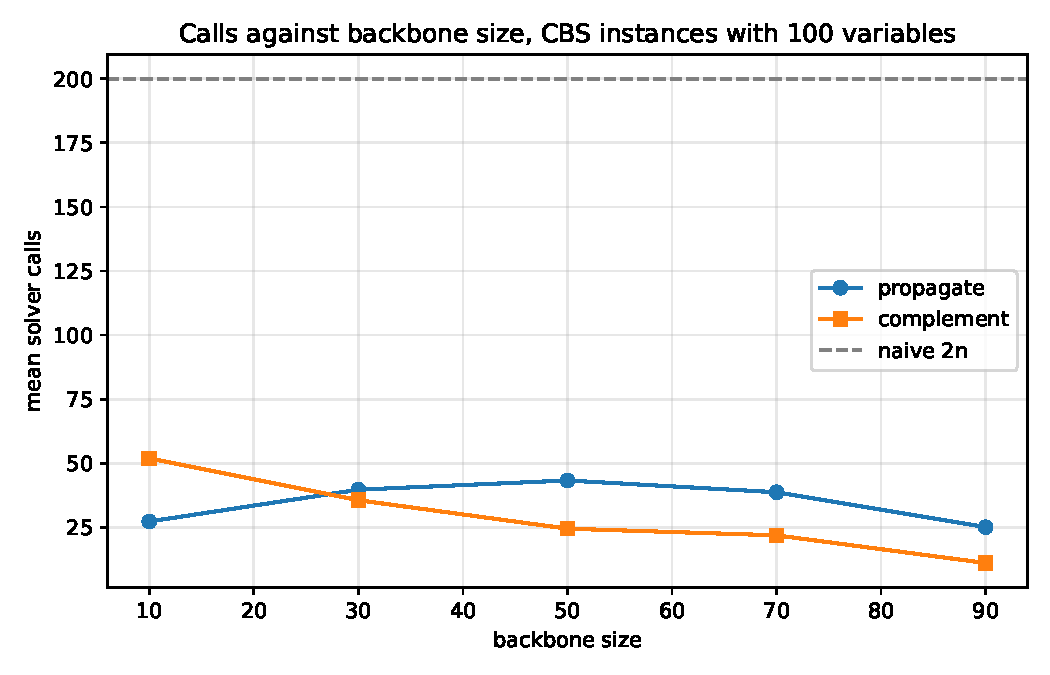
\includegraphics[width=0.72\textwidth]{figures/calls_vs_backbone.pdf}
\caption{Mean calls against backbone size on the CBS instances, with the naive
baseline for comparison.}
\label{fig:cbs}
\end{figure}

Figure~\ref{fig:cbs} shows the same numbers, and the two shapes are easier to
compare there: \code{complement} decreasing throughout, \code{propagate}
humped, and the two crossing between ten and thirty forced variables. Both
remain far below the flat naive line at 200 for every backbone size.

\subsection*{Per family}

\begin{table}[H]
\centering
\begin{tabular}{lrrrrrr}
\toprule
family & vars & backbone & \code{propagate} & \code{complement} & naive & free \\
\midrule
\code{uf20-91} & 20 & 12.8 & 8.4 & 4.8 & 40 & 7 \\
\code{uf50-218} & 50 & 38.8 & 18.0 & 8.4 & 100 & 26 \\
\code{flat30-60} & 90 & 0.0 & 12.6 & 24.0 & 180 & 0 \\
\code{BMS\_k3\_n100\_m429} & 100 & 29.0 & 34.6 & 41.8 & 200 & 8 \\
\code{RTI\_k3\_n100\_m429} & 100 & 29.0 & 34.2 & 34.0 & 200 & 8 \\
\code{uf100-430} & 100 & 30.0 & 33.0 & 31.2 & 200 & 10 \\
\code{flat50-115} & 150 & 0.0 & 10.4 & 25.8 & 300 & 0 \\
\code{ais} & 155 & 1.2 & 28.0 & 35.8 & 310 & 0 \\
\code{flat100-239} & 300 & 0.0 & 13.8 & 37.4 & 600 & 0 \\
\code{sw100-8-p0-c5} & 500 & 0.0 & 13.0 & 17.0 & 1\,000 & 0 \\
\code{blocksworld} & 1\,644 & 1590.7 & 77.9 & 5.1 & 3\,289 & 1\,517 \\
\code{logistics} & 1\,881 & 559.2 & 744.2 & 739.5 & 3\,762 & 142 \\
\bottomrule
\end{tabular}
\caption{Mean calls per instance by family, CBS omitted as it appears in
Table~\ref{tab:cbs}. Every column is a mean over the instances of the family,
including the number of variables and the naive cost derived from it. The free
column is the mean number of backbones obtained by propagation under
\code{propagate}.}
\label{tab:family}
\end{table}

The graph colouring families \code{flat30-60}, \code{flat50-115},
\code{flat100-239} and \code{sw100-8-p0-c5} have no backbones at all, since
permuting the colours maps any solution to another and no variable keeps its
value across every model. This is the best case for \code{propagate}: every
candidate is refuted by a model, each model prunes many at once, and no call
is spent confirming. It needs $13.0$ calls on the 500 variable instance
against $17.0$ for \code{complement} and $1\,000$ naive, and the margin widens
with size, $13.8$ against $37.4$ on \code{flat100-239}.

\code{blocksworld} is the opposite case and the widest gap in the table. Its
instances are almost fully forced, $1590.7$ backbones out of $1644$ variables,
so confirmation is the whole job: \code{complement} confirms in bulk and needs
$5.1$ calls, \code{propagate} commits one backbone at a time and needs $77.9$,
against $3\,289$ naive. Propagation supplies $1\,517$ of those backbones
without a call.

The two extremes give the rule. Each algorithm eliminates candidates in one of
the two available ways and wins where that way carries the instance:
\code{propagate} where most candidates are refutable, \code{complement} where
most are backbones. Hence the near equal totals of Table~\ref{tab:cost} over
per family figures that differ tenfold in both directions.

\begin{figure}[H]
\centering
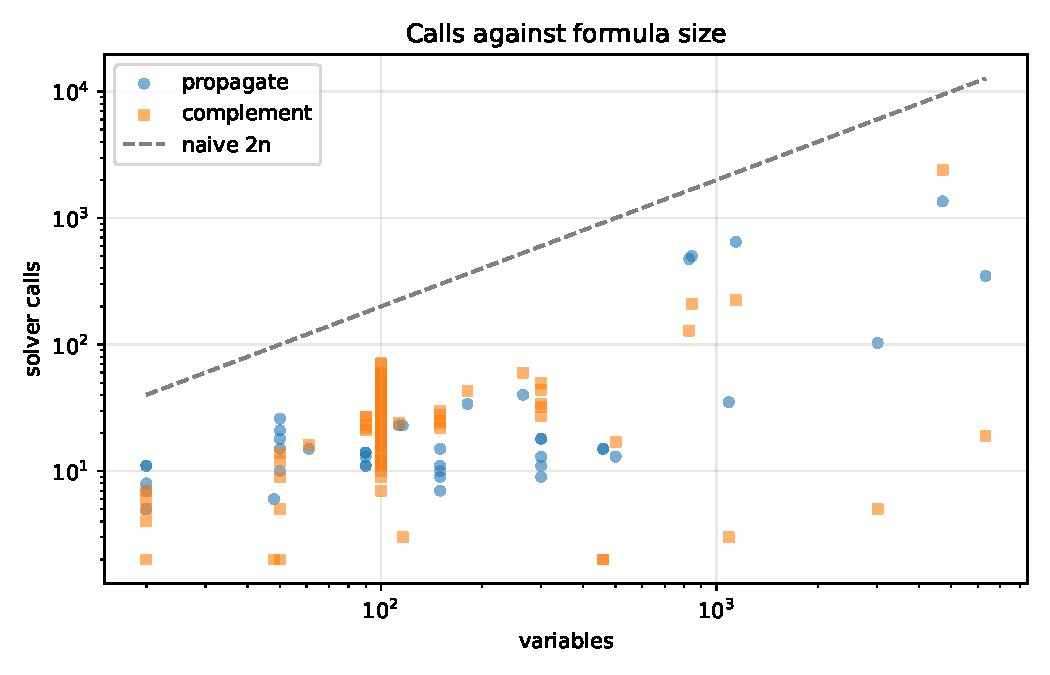
\includegraphics[width=0.72\textwidth]{figures/calls_vs_size.pdf}
\caption{Calls against the number of variables, both axes logarithmic, with
the naive $2n$ line.}
\label{fig:size}
\end{figure}

Figure~\ref{fig:size} plots every run against formula size. Both algorithms
sit below the naive diagonal everywhere, but neither is a function of size:
\code{propagate} spends $0.03$ to $0.59$ calls per variable, median $0.32$,
and \code{complement} $0.002$ to $0.71$, median $0.24$. Both scatter over more
than an order of magnitude at a given $n$, so what an instance costs is
decided by how much of it is forced rather than by how large it is.

\begin{figure}[H]
\centering
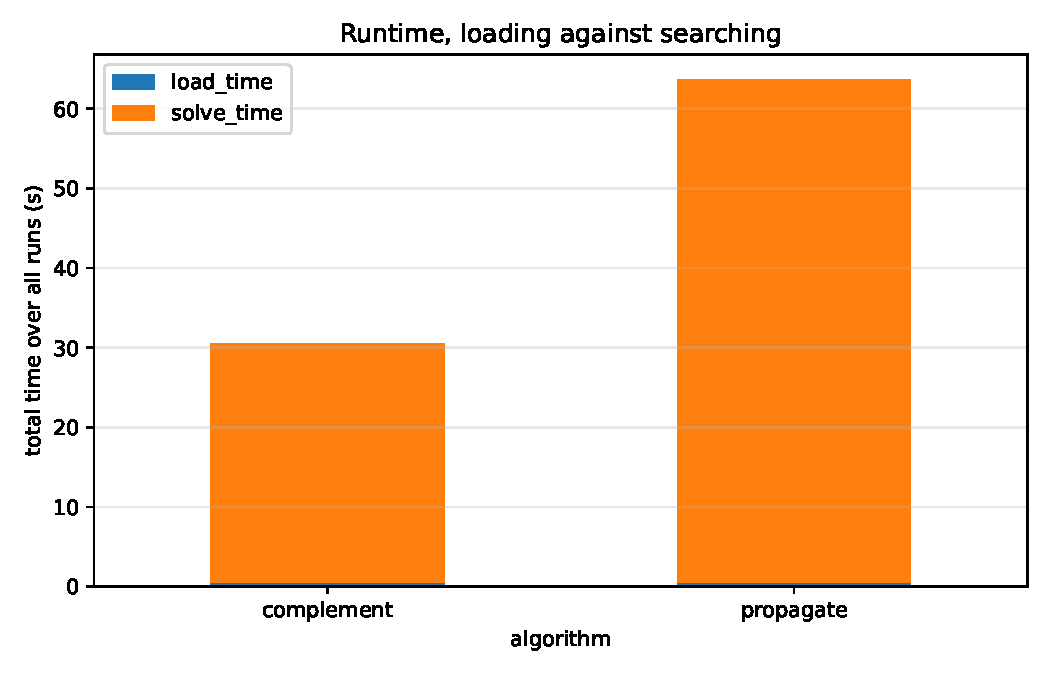
\includegraphics[width=0.72\textwidth]{figures/runtime.pdf}
\caption{Total time over all runs, split into loading the formula and
searching.}
\label{fig:runtime}
\end{figure}

Time does not follow the call count. Loading is negligible for both, since
each loads the formula once and then works incrementally, so the search
accounts for almost everything. \code{propagate} makes $11\%$ more calls than
\code{complement} but spends twice as long searching, $63.1$ seconds against
$30.1$, so its calls are the dearer ones: assuming one literal leaves the
solver most of the space to explore, while a blocking clause rules out a whole
block of assignments and reaches an answer sooner.

\subsection*{Code}

All code is in \code{backbones/code/} and is available in the
repository~\cite{repo}.

\begin{itemize}
  \item \code{backbone.py} holds the reader for DIMACS files, the unit
  propagation used for free backbones, and the two algorithms/variants. Only
  calls to the solver are counted here.

  \item \code{verify.py} holds the independent checking, including the routine
  that recomputes a backbone from scratch. Everything in it creates its own
  solver instances and its own counters, so a call made while verifying can
  never reach the measured results. Nothing in it is used by the algorithms.

  \item \code{bench.py} runs the sweep and records the calls, the backbone
  size, the free literals and the times.

  \item \code{test\_backbone.py} contains the correctness checks: the small
  formulas, the unsatisfiable case, the soundness of the propagated literals,
  the exhaustive verification and the CBS ground truth.

  \item \code{experiments.ipynb} runs everything and writes \code{results.csv},
  \code{verification.csv} and the figures used here. The full verification is a
  separate section at the end so that it stays out of the measurements.
\end{itemize}

The benchmark instances are in \code{benchmarks\_allSAT/}, one level above the
task folders so that other tasks can use the same set.

\subsection*{Summary}

Both algorithms find the correct backbones. This is confirmed by inspection on
small formulas, by the stated backbone sizes of the CBS family on 150 runs,
and most completely by recomputing the backbone of every instance from scratch
and comparing it literal by literal, which agreed in all 262 comparisons with
nothing missing and nothing spurious. The two algorithms also agree with each
other on all 131 instances.

On the quantity the task asks to minimise both algorithms do well and neither
wins outright. \code{complement} used $6\,367$ solver calls and
\code{propagate} $7\,083$, where the naive algorithm would have used
$64\,410$, reductions of ten and nine times. The single most valuable step is
the one the task points at, using the models the solver returns: one model at
the start removes half of the $2n$ literals immediately, and every further
model removes every candidate it falsifies, so \code{propagate} never pays
one call per variable.

The totals hide two different algorithms.
Candidates are eliminated in one of two ways, refuted by a model or confirmed
by an unsatisfiable call, and each design is built around one of them.
\code{propagate} lets models do the pruning and pays for confirmation, so it
is cheapest where there is little to confirm: on graph colouring with no
backbones at all it takes $13.0$ calls on a 500 variable instance.
\code{complement} confirms a whole block in one round and pays for refutation,
so it is cheapest where almost everything is forced: on \code{blocksworld} it
finds more than fifteen hundred backbones in $5.1$ calls where
\code{propagate} needs $77.9$. On the CBS family, where the size of the
backbone is controlled directly, this shows up as a hump in the cost of
\code{propagate} with its peak in the middle, against a steady fall for
\code{complement}.

Unit propagation is a smaller but genuinely free gain, producing $13\,477$
backbones across the experiment at no solver cost, and it is most useful on
the structured instances where committing one backbone cascades into many.

\clearpage

\begin{thebibliography}{9}

\bibitem{satlib}
H. Hoos, T. St\"utzle, \emph{SATLIB: An Online Resource for Research on SAT}.
\url{https://www.cs.ubc.ca/~hoos/SATLIB/benchm.html}

\bibitem{cbs}
J. Singer, I. P. Gent, A. Smaill, \emph{Backbone Fragility and the Local
Search Cost Peak}, Journal of Artificial Intelligence Research, vol. 12,
pp. 235--270, 2000.
\url{https://doi.org/10.1613/jair.711}

\bibitem{pysat}
A. Ignatiev, A. Morgado, J. Marques-Silva,
\emph{PySAT: A Python Toolkit for Prototyping with SAT Oracles}, SAT 2018.
\url{https://pysathq.github.io}

\bibitem{cadical}
A. Biere, \emph{CaDiCaL}.
\url{http://fmv.jku.at/cadical}

\bibitem{repo}
Z. Ahmetovic, source code for this task.
\url{https://github.com/inferno73/SAT-solver-NAIL094}

\end{thebibliography}

\end{document}
